\chapter*{ПРИЛОЖЕНИЕ A}
\addcontentsline{toc}{chapter}{ПРИЛОЖЕНИЕ A}

\begin{figure}[ht!]\centering
	
\includegraphics[width=\linewidth]{pres_1}
	\caption{Титульный слайд (слайд 1)}
\end{figure}

\begin{figure}[ht!]\centering
	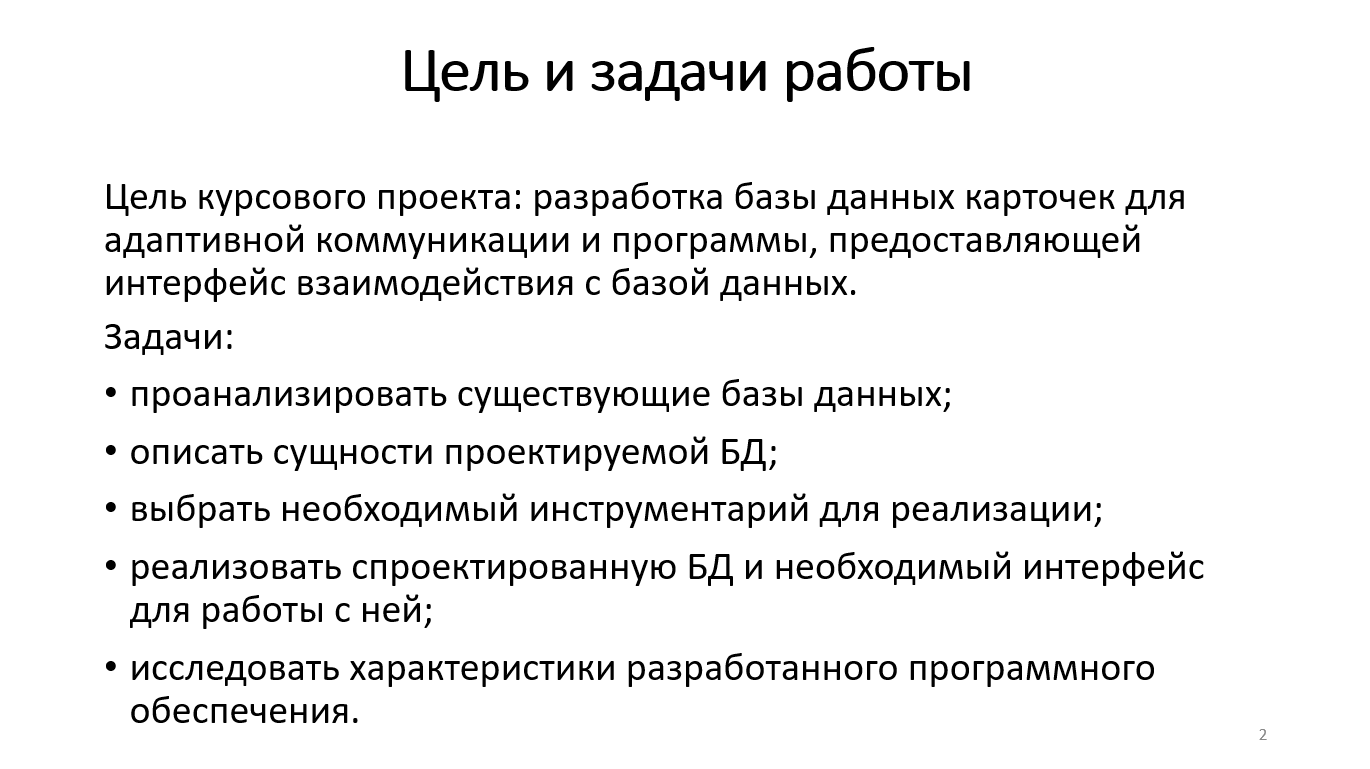
\includegraphics[width=\linewidth]{pres_2}
	\caption{Цель работы (слайд 2)}
\end{figure}

\begin{figure}[ht!]\centering
	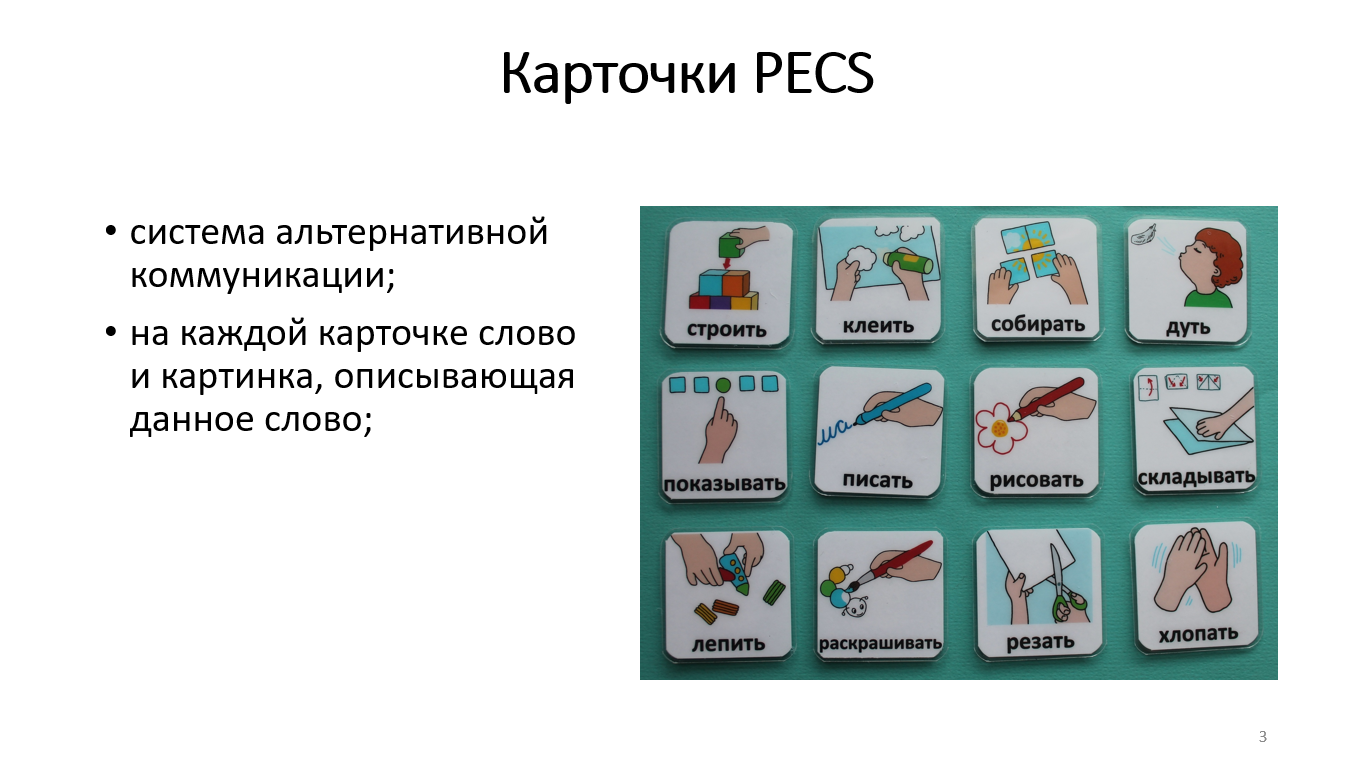
\includegraphics[width=\linewidth]{pres_3}
	\caption{Задачи курсового проекта (слайд 3)}
\end{figure}

\begin{figure}[ht!]\centering
	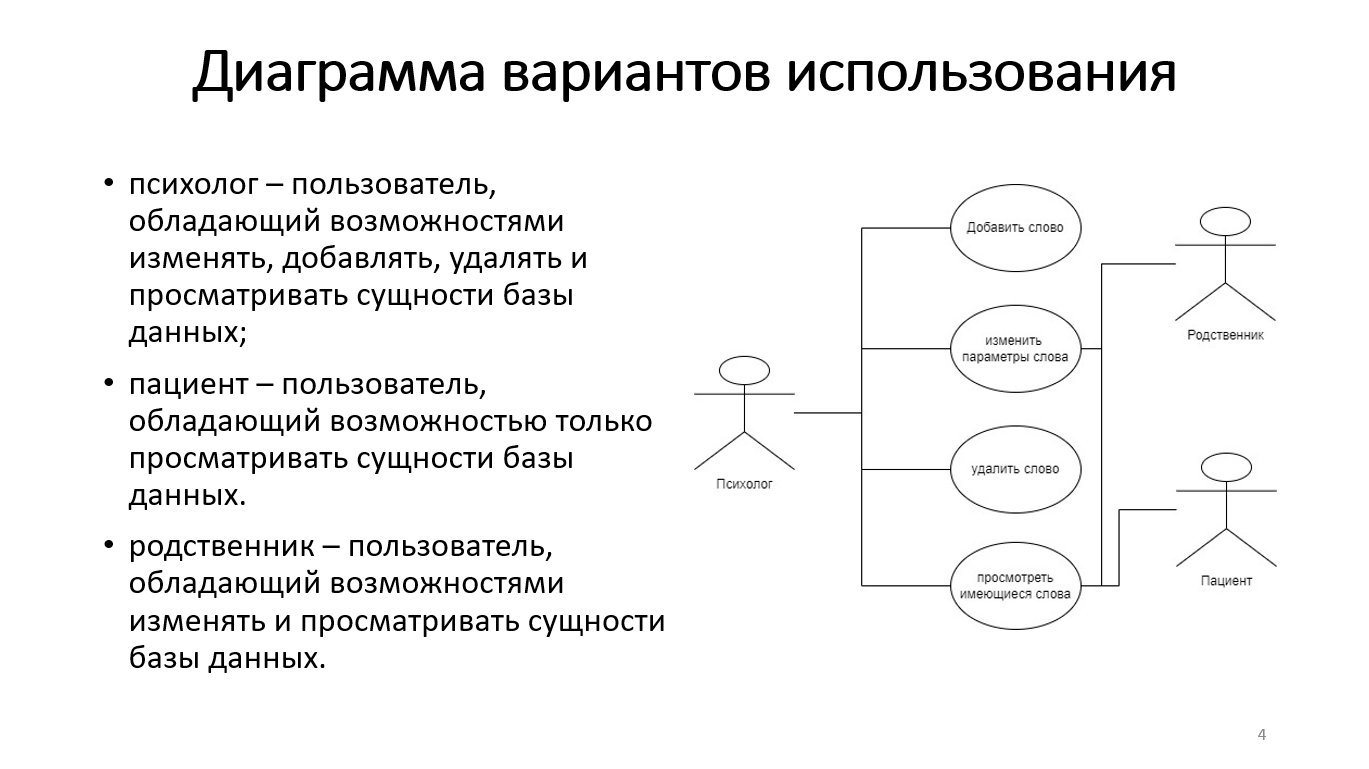
\includegraphics[width=\linewidth]{pres_4}
	\caption{Анализ алгоритмов отображения (слайд 4)}
\end{figure}

\begin{figure}[ht!]\centering
	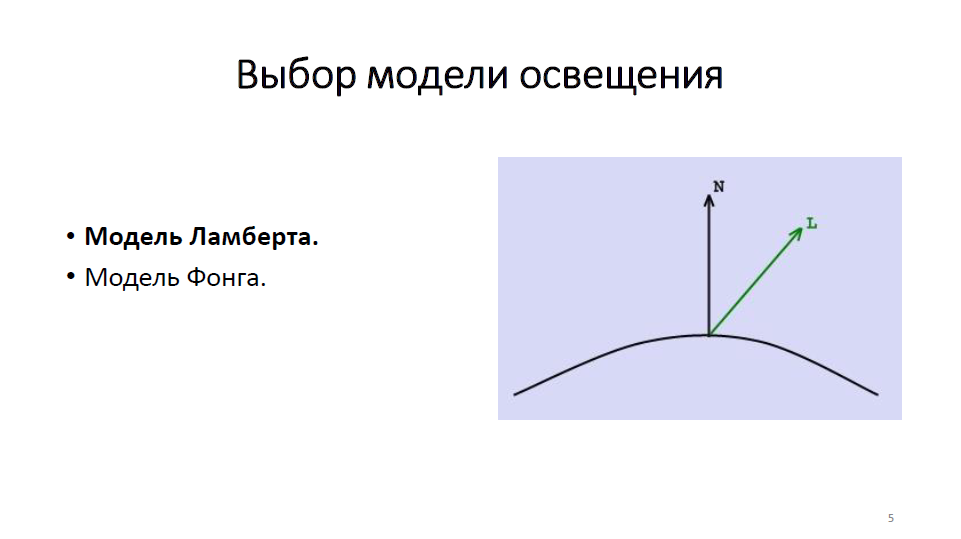
\includegraphics[width=\linewidth]{pres_5}
	\caption{Выбор модели освещения (слайд 5)}
\end{figure}

\begin{figure}[ht!]\centering
	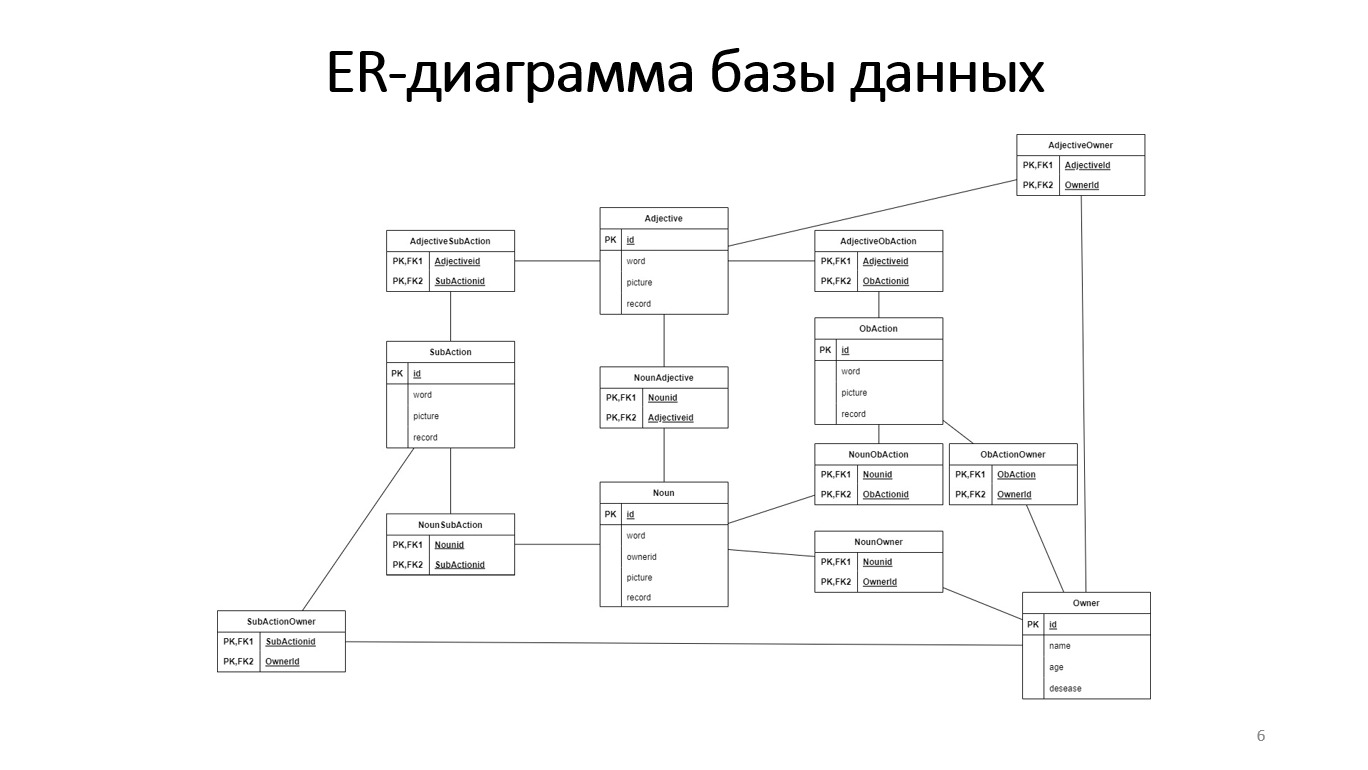
\includegraphics[width=\linewidth]{pres_6}
	\caption{Закон движения частиц (слайд 6)}
\end{figure}

\begin{figure}[ht!]\centering
	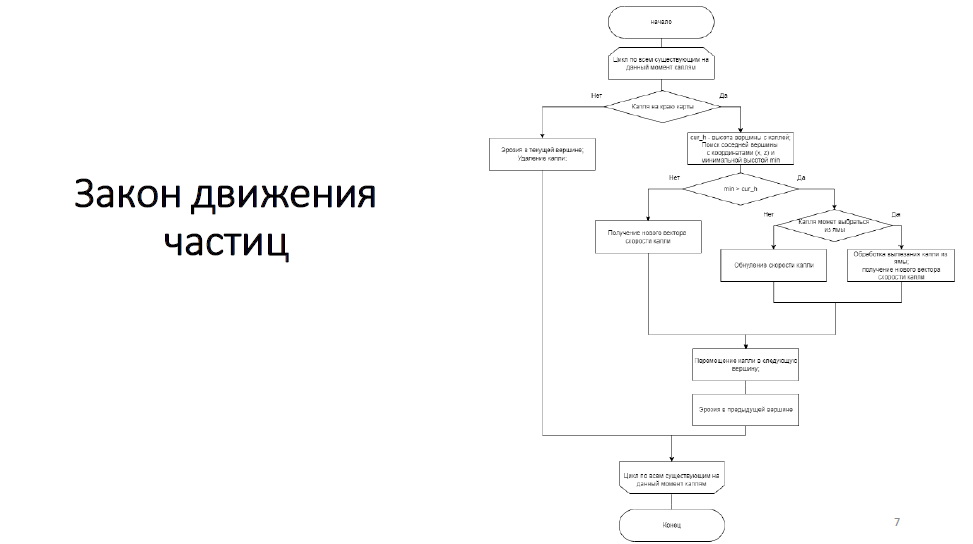
\includegraphics[width=\linewidth]{pres_7}
	\caption{Закон движения частиц (слайд 7)}
\end{figure}

\begin{figure}[ht!]\centering
	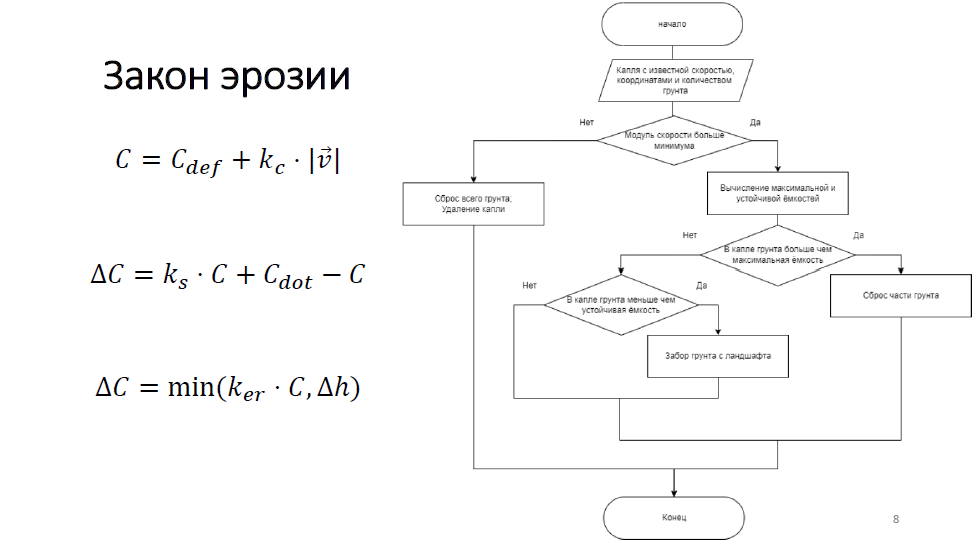
\includegraphics[width=\linewidth]{pres_8}
	\caption{Закон эрозии (слайд 8)}
\end{figure}

\begin{figure}[ht!]\centering
	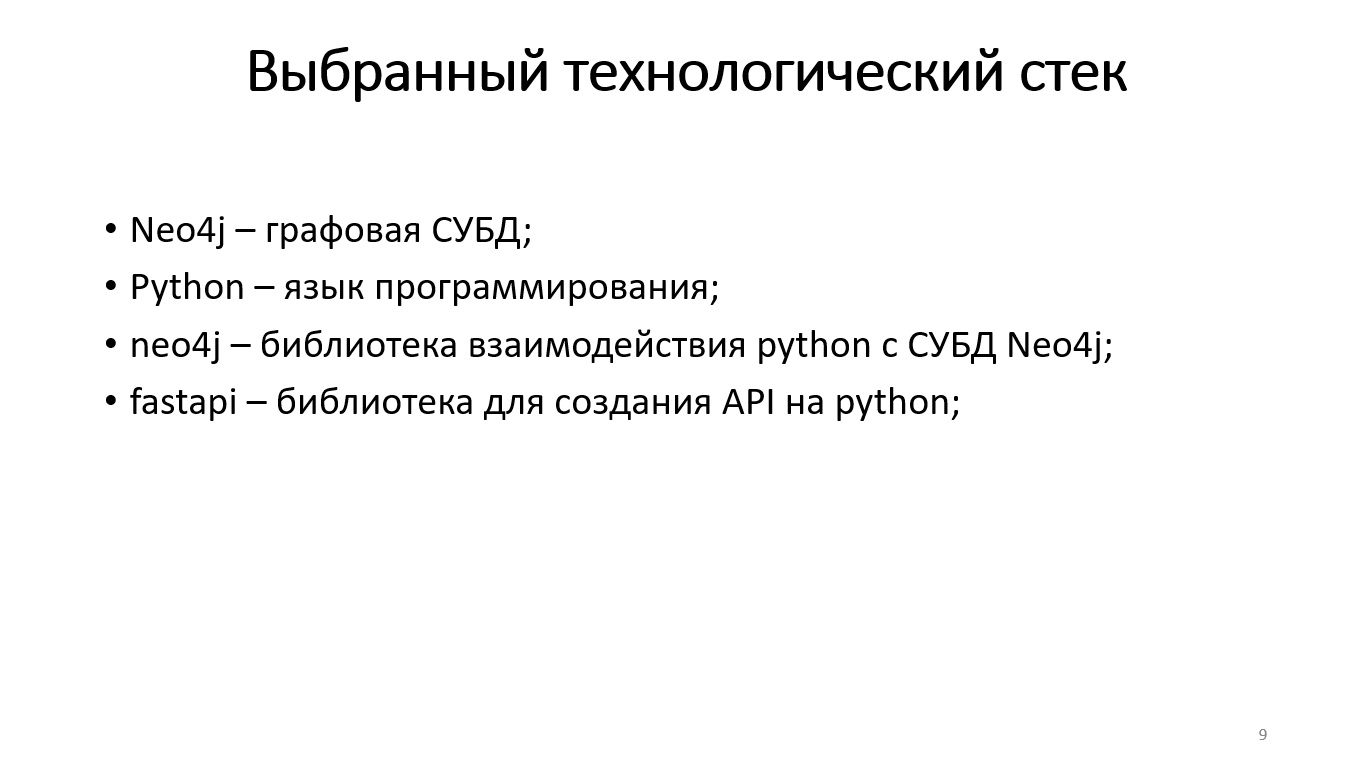
\includegraphics[width=\linewidth]{pres_9}
	\caption{Интерфейс главного окна (слайд 9)}
\end{figure}

\begin{figure}[ht!]\centering
	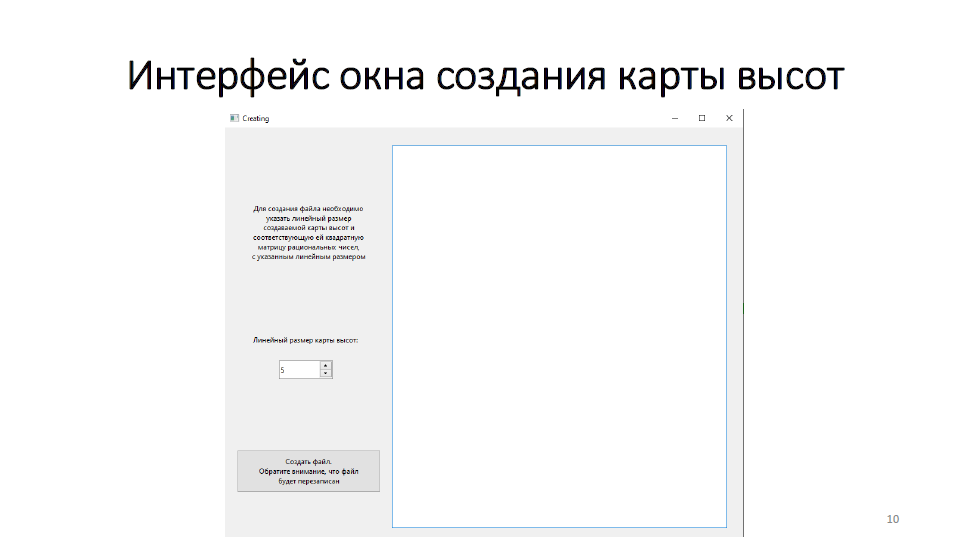
\includegraphics[width=\linewidth]{pres_10}
	\caption{Интерфейс окна создания карты высот (слайд 10)}
\end{figure}

\begin{figure}[ht!]\centering
	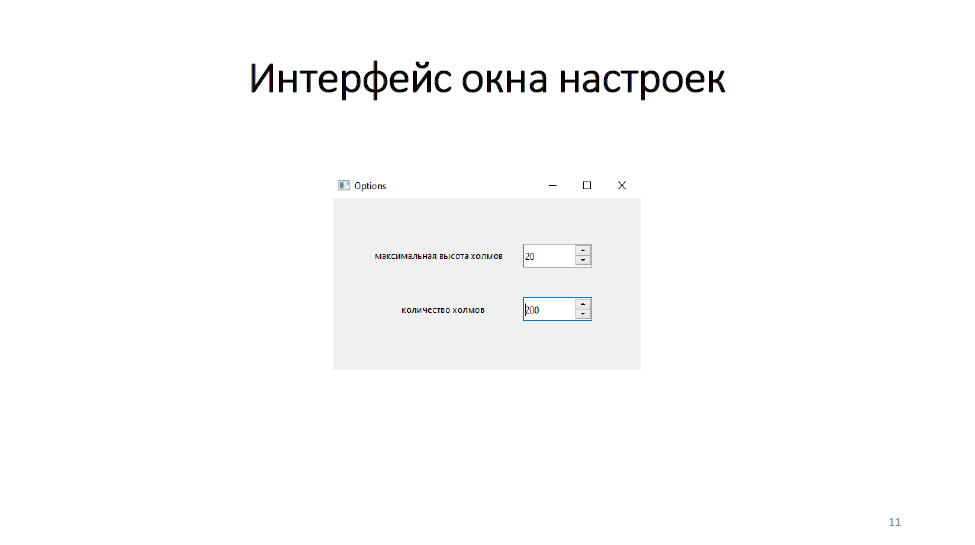
\includegraphics[width=\linewidth]{pres_11}
	\caption{Интерфейс окна настроек (слайд 11)}
\end{figure}

\begin{figure}[ht!]\centering
	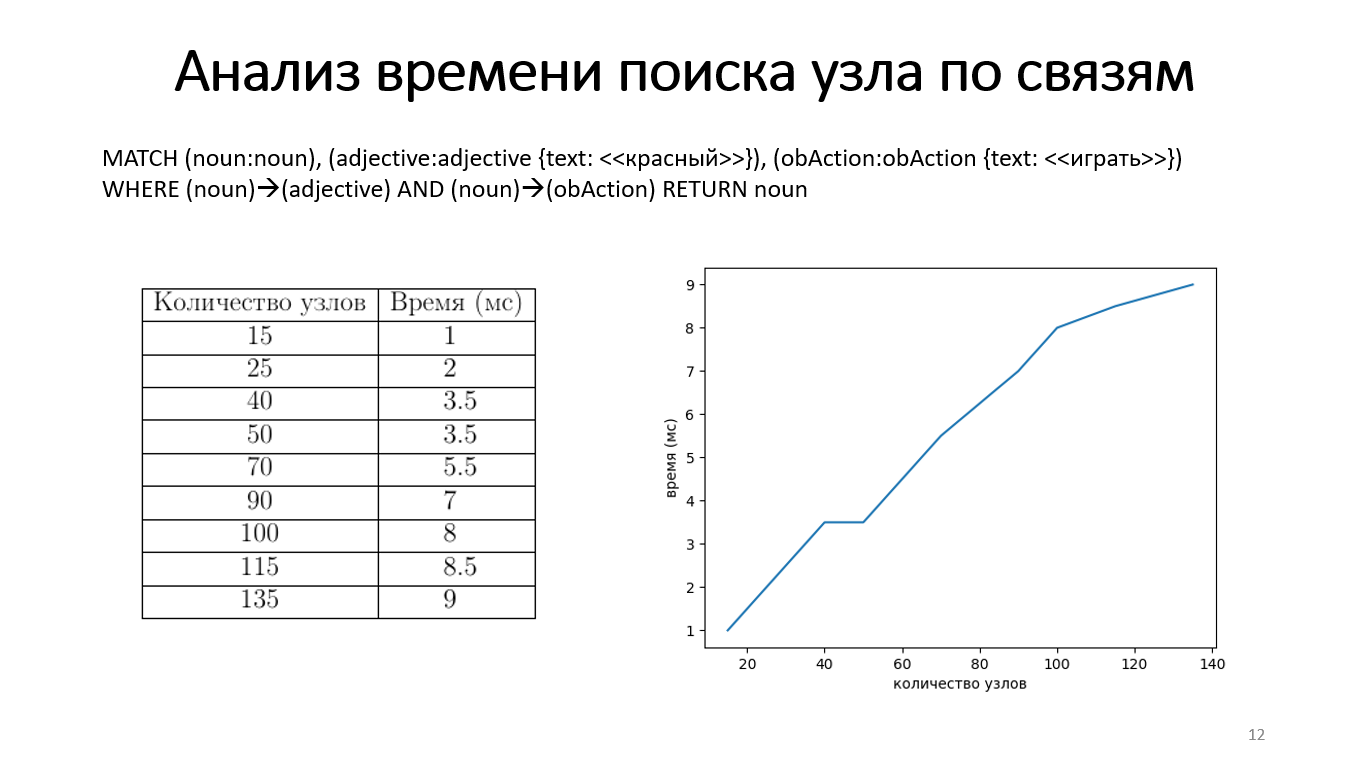
\includegraphics[width=\linewidth]{pres_12}
	\caption{Пример работы программы (слайд 12)}
\end{figure}

\begin{figure}[ht!]\centering
	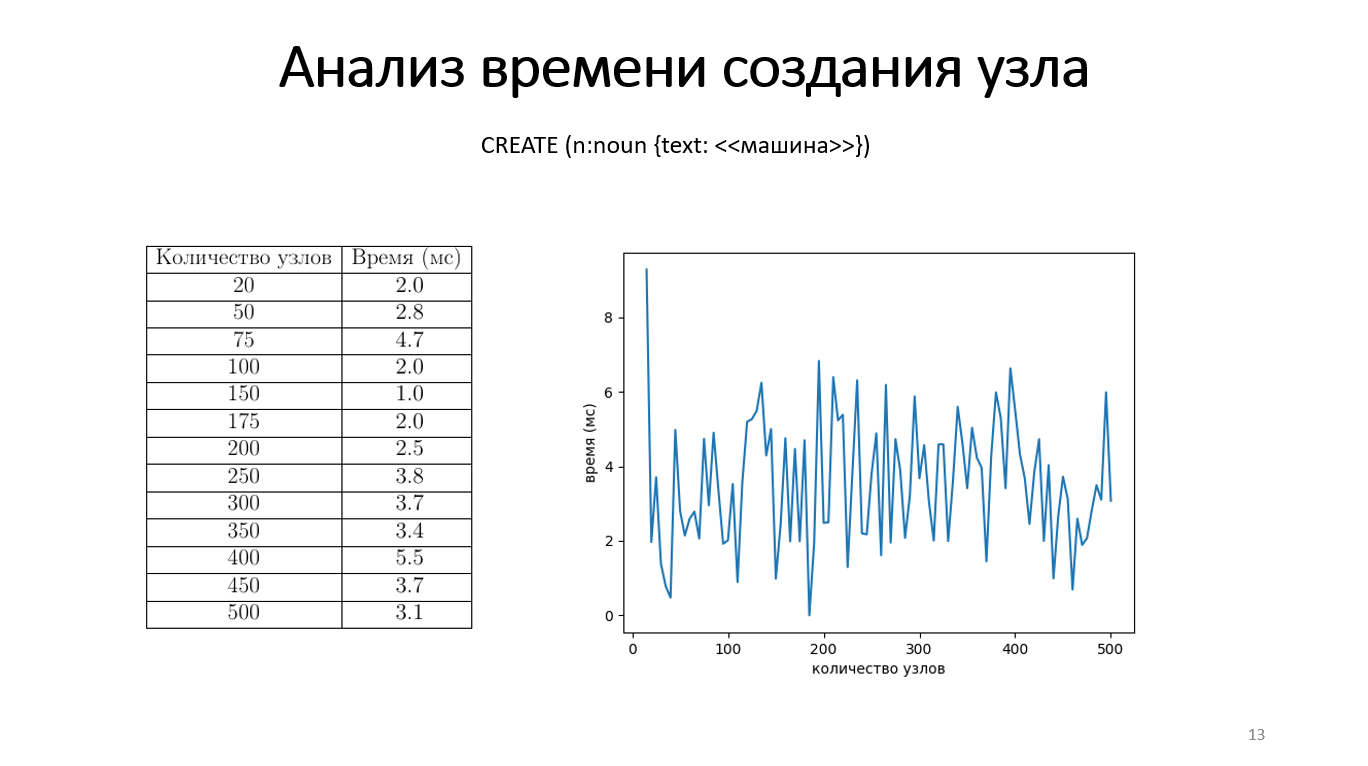
\includegraphics[width=\linewidth]{pres_13}
	\caption{Заключение (слайд 13)}
\end{figure}


